\subsection {Требования к аппаратному обеспечению}
Минимальные системные требования:

\begin{itemize}
\item процессор 1ГГц Pentium 4;
\item оперативная память 512 Мб;
\item место на жёстком диске -- 9 Гб.
\end{itemize}

\subsection {Требования к программному обеспечению}
Для корректной работы разрабатываемого программного комплекса на компьютере должна быть установлена операционная система Debian Squeeze или выше, данная система должна иметь набор библиотек Qt, CMake и DV.

\subsection {Выбор формата выходных файлов}
Для вывода результата был выбран формат файла HDF5. 

Hierarchical Data Format, HDF (Иерархический формат данных) — название формата файлов, разработанного для хранения большого количества цифровой информации.

HDF5 — современная версия формата содержит иерархию из двух основных типов объектов:
HDF-Structure-Example
\begin{enumerate}
\item Datasets — наборы данных, многомерные массивы объектов одного типа
\item Groups — группы, являются контейнерами для наборов данных и других групп
\end{enumerate}
    
Содержимое файлов HDF5 организовано подобно иерархической файловой системе, и для доступа к данным применяются пути, сходные с POSIX-синтаксисом, например, /path/to/resource. Метаданные хранятся в виде набора именованных атрибутов объектов.\cite{hdf5}
\begin{figure}
\centering
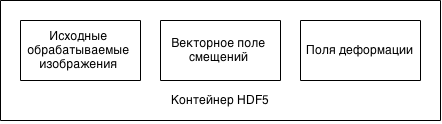
\includegraphics[width=0.7\linewidth]{images/structHDF5}
\caption{Структура HDF5 файла}
\label{fig:structHDF5}
\end{figure}

Структура сохранения результатов работы представлена на рисунке \ref{fig:structHDF5}

Под блоком исходные обрабатываемые изображения подразумевается входная пара изображений(левая, правая) в форматах png, bmp, jpg, tiff и др. В выходном файле они представлены двумя слоями: ``left'' и ``right''. Они необходимы для удобства просмотра в программе Defomation-Analysis. Программа Defomation-Analysis умеет выводить отдельные слои и накладывать их друг на друга.

Блок векторное поле смешений является бинарным файлом, формата ``vf''. Слой содержит информацию о размерах исходного изображения, координаты векторов смещений и векторы в формате double (формула \ref{eq:lucas}).

Блок поля деформации также является бинарным файлом и содержит слои деформации:
\begin{enumerate}
\item $\varepsilon_{xx}$ - продольная (формула \ref{eq:e_xx});
\item $\varepsilon_{yy}$ - поперечная (формула \ref{eq:e_yy});
\item $\varepsilon_{xy}$ - сдвиговая (формула \ref{eq:e_xy});
\item $w_{i}$ - поворотная (формула \ref{eq:w_z});
\item $\gamma_z$ - интенсивность деформации сдвига (формула \ref{eq:gamma_i}).
\end{enumerate}s